\documentclass[11pt]{amsart}
\usepackage{hyperref}
\usepackage{geometry}                % See geometry.pdf to learn the layout options. There are lots.
\geometry{letterpaper}                   % ... or a4paper or a5paper or ... 
%\geometry{landscape}                % Activate for for rotated page geometry
\usepackage[parfill]{parskip}    % Activate to begin paragraphs with an empty line rather than an indent
\usepackage{graphicx}
\usepackage{amssymb}
\usepackage[all]{xy}
\usepackage{epstopdf}
\usepackage{color}
\DeclareGraphicsRule{.tif}{png}{.png}{`convert #1 `dirname #1`/`basename #1 .tif`.png}


% these packages make it easy to include figures in the text. 
\usepackage{float}
\restylefloat{figure}
% newcommand
\newcommand{\ip}[1]{\left\langle #1\right\rangle}



\begin{document}
{\Large Name: Philip Pham}  \\
\begin{center}
\Large AMATH 515 \hskip 2in Homework Set 4\\
{\bf Due: Wednesday, March 18th, on Canvas}. 
\end{center}
\bigskip
\begin{enumerate}

\item  Prove the following identity for $\alpha \in \mathbb{R}$:
\[
\|\alpha x + (1-\alpha) y\|^2 + \alpha(1-\alpha) \|x-y\|^2 = \alpha \|x\|^2 + (1-\alpha) \|y\|^2.
\]

\begin{proof}
  This follows from the fact that
  $\| u - v \|^2 = \langle u, u \rangle + \langle v, v \rangle -
  2\langle u, v \rangle$.

  With some algebra,
  \begin{align*}
    \|\alpha x + (1-\alpha) y\|^2 + \alpha(1-\alpha) \|x-y\|^2
    &= \alpha^2 \langle x, x \rangle + (1-\alpha)^2 \langle y, y \rangle
      + 2\alpha(1-\alpha)\langle x, y \rangle \\
    & + \alpha(1-\alpha)\langle x, x \rangle + \alpha(1-\alpha)\langle y, y \rangle
      -2\alpha(1-\alpha)\langle x, y \rangle\\
    &= \alpha \langle x, x \rangle + (1-\alpha)\left[1 - \alpha + \alpha\right]\langle y, y \rangle \\
    &=\alpha \|x\|^2 + (1-\alpha) \|y\|^2.
  \end{align*}
\end{proof}


\item An operator $T$ is {\it nonexpansive} if  $\|Tx - Ty\| \leq \|x - y\|$ for all $(x,y)$. 
For any such nonexpansive operator $T$, define 
\[
T_\lambda = (1-\lambda)I + \lambda T. 
\]
\begin{enumerate}
\item Show that $T_\lambda$ and $T$ have the same fixed points.
  \begin{proof}
    Suppose that $Tx = x$. Then, it's easy to see that
    \begin{align*}
      T_\lambda x
      &= \left((1-\lambda)I + \lambda T\right)x \\
      &= (1-\lambda)Ix + \lambda Tx \\
      &= (1-\lambda)x + \lambda x = x.
    \end{align*}

    Similarly, suppose $T_\lambda y = y$. If $\lambda \neq 0$, then
    $T = \lambda^{-1}\left(T_\lambda - (1-\lambda)I\right)$, and
    \begin{align*}
      Ty
      &= \lambda^{-1}\left(T_\lambda - (1-\lambda)I\right)y \\
      &=\lambda^{-1}\left(T_\lambda y -  (1-\lambda)Iy\right) \\
      &=\lambda^{-1}\left(y - \left(1 - \lambda\right)y\right) \\
      &=\lambda^{-1}\left(\lambda y\right) = y.
    \end{align*}

    Thus, when $\lambda \neq 0$, the set of fixed points are the same. When
    $\lambda = 0$, the set of fixed points of $T$ is a subset of the fixed
    points of $T_\lambda = I$.
  \end{proof}
\item Use problem 1 to show 
\[
\|T_\lambda z - \overline z\|^2 \leq \|z-\overline z\|^2 - \lambda(1-\lambda) \|z - Tz\|^2.
\]
where $\overline z$ is any fixed point of $T$, i.e. $T\overline z = \overline z$.

\begin{proof}
  We first apply the definition of $T_\lambda$. Next, we use the identity in
  problem 1. Then, we use that $\overline z$ is a fixed point of $T$. Finally,
  we use the nonexpansive property of $T$ for the inequality.
  \begin{align*}
    \|T_\lambda z - \overline z\|^2
    &=
      \|(1-\lambda)z + \lambda Tz - \lambda\overline z - (1-\lambda)\overline z\|^2 \\
    &=
      \|(1-\lambda)(z - \overline z) + \lambda (Tz - \overline z) \|^2 \\
    &=
      \|(1-\lambda)(z - \overline z) + \lambda (Tz - \overline z) \|^2
      + \lambda(1-\lambda)(z - Tz)
      - \lambda(1-\lambda)(z - Tz) \\
    &= (1-\lambda)\|z - \overline z\|^2 + \lambda \|Tz - \overline z\|^2
      - \lambda(1-\lambda)(z - Tz) \\
    &= (1-\lambda)\|z - \overline z\|^2 + \lambda \|Tz - T\overline z\|^2
      - \lambda(1-\lambda)(z - Tz) \\
    &\leq
      (1-\lambda)\|z - \overline z\|^2 + \lambda \|z - \overline z\|^2
      - \lambda(1-\lambda)(z - Tz) \\
    & = \|z - \overline z\|^2 - \lambda(1-\lambda)(z - Tz).
  \end{align*}
  Note that the inequality is only valid when $\lambda \geq 0$.
\end{proof}

\end{enumerate}

\item An operator $T$ is {\it firmly nonexpansive} when it satisfies 
\[
\|Tx - Ty\|^2 + \|(I-T) x - (I-T)y\|^2 \leq \|x-y\|^2. 
\]


\begin{enumerate}
\item Show $T$ is firmly nonexpansive if and only if 
\[
\langle x-y, Tx - Ty \rangle \geq \|Tx - Ty\|^2. 
\]

\begin{proof}
  Suppose $T$ is firmly nonexpansive.
  \begin{align*}
    \|Tx - Ty\|^2
    &+ \|(I-T) x - (I-T)y\|^2 \leq \|x-y\|^2 \\
    &\Leftrightarrow \|Tx - Ty\|^2 + \|(x-y)- (T x - T y)\|^2 \leq \|x-y\|^2 \\
    &\Leftrightarrow
      \|Tx - Ty\|^2 + \|(x-y)- (T x - T y)\|^2 \leq \|x-y\|^2 \\
    &\Leftrightarrow
      \|Tx - Ty\|^2 + \|x-y\|^2 + \|T x - T y)\|^2
      - 2\langle x - y, T x - T y\rangle \leq \|x-y\|^2 \\
    &\Leftrightarrow
      2\|Tx - Ty\|^2 \leq 2\langle x - y, T x - T y\rangle \\
    &\Leftrightarrow
      2\|Tx - Ty\|^2 \leq 2\langle x - y, T x - T y\rangle \\
    &\Leftrightarrow
      \langle x - y, T x - T y\rangle  \geq \|Tx - Ty\|^2,
  \end{align*}
  which is the desired result.
\end{proof}
\item Show $T$ is firmly nonexpansive if and only if 
\[
\langle Tx - Ty, (I-T)x - (I-T)y \rangle \geq 0. 
\]

\begin{proof}
  This follows from the previous result in part (a) and the bilinearity of the
  inner product:
  \begin{align*}
    \text{$T$ is firmly nonexpansive}
    &\Leftrightarrow \langle x-y, Tx - Ty \rangle \geq \|Tx - Ty\|^2 \\
    &\Leftrightarrow \langle x-y, Tx - Ty \rangle - \|Tx - Ty\|^2 \geq  0 \\
    &\Leftrightarrow \langle x-y, Tx - Ty \rangle - \langle Tx - Ty, Tx - Ty \rangle \geq  0 \\
    &\Leftrightarrow \langle x-y - (Tx - Ty), Tx - Ty \rangle \geq  0 \\
    &\Leftrightarrow \langle (I - T)x - (I - T)y, Tx - Ty \rangle \geq  0 \\
    &\Leftrightarrow \langle Tx - Ty, (I - T)x - (I - T)y \rangle \geq  0,
  \end{align*}
  which is the desired result.
\end{proof}

\item Suppose that $S = 2T - I$. Let 
\[
\mu = \|Tx - Ty\|^2 + \|(I-T)x - (I-T)y\|^2 - \|x-y\|^2
\]
and let 
\[
\nu = \|Sx - Sy\|^2 - \|x-y\|^2.
\]
Show that $2\mu = \nu$ (you may find it helpful to use problem (1)). Conclude that 
$T$ is firmly nonexpansive exactly when $S$ is nonexpansive.

\begin{proof}
  To prove $\nu = 2\mu$, there's a lot of algebra:
  \begin{align*}
    \nu &=\|Sx - Sy\|^2 - \|x-y\|^2
    = \|(Tx - Ty) - [(I - T)x - (I - T)y]\|^2  - \|x-y\|^2 \\    
    &= \|Tx - Ty\|^2 + \|(I - T)x - (I - T)y\|^2
      - 2\langle Tx - Ty, (I - T)x - (I - T)y\rangle - \|x-y\|^2.
  \end{align*}

  We focus on the $-2\langle Tx - Ty, (I - T)x - (I - T)y\rangle$ term.
  \begin{align*}
    &-2\langle Tx - Ty, (I - T)x - (I - T)y\rangle \\
    &= \langle Tx - Ty, Tx - Ty \rangle + \langle Tx - Ty, Tx - Ty \rangle
      - 2\langle Tx - Ty, x - y \rangle \\
    &= \langle Tx - Ty, Tx - Ty \rangle + \langle Tx - Ty, Tx - Ty \rangle
      - 2\langle Tx - Ty, x - y \rangle + \langle x - y, x - y \rangle - \langle x - y, x - y \rangle \\
    &= \| Tx - Ty \|^2 + \langle Tx - Ty, Tx - Ty \rangle
      - 2\langle Tx - Ty, x - y \rangle + \langle x - y, x - y \rangle - \langle x - y, x - y \rangle \\
    &= \| Tx - Ty \|^2 + \| (Tx - Ty) - (x-y) \|^2 - \| x - y \|^2 \\
    &= \| Tx - Ty \|^2 + \| (I - T)x - (I- T)y\|^2 - \| x - y \|^2 \\
  \end{align*}
  where we have completed the square to get the $\| (Tx - Ty) - (x-y) \|^2$
  term.

  Substituting back into the first equation, we have that
  \begin{align*}
    \nu
    &= \|Tx - Ty\|^2 + \|(I - T)x - (I - T)y\|^2 \\
    &+ \left[\| Tx - Ty \|^2 + \| (I - T)x - (I- T)y\|^2 - \| x - y \|^2\right] - \|x-y\|^2 \\
    &= 2\|Tx - Ty\|^2 + 2\|(I - T)x - (I - T)y\|^2 - 2\| x - y \|^2 \\
    &= 2\left[\|Tx - Ty\|^2 + \|(I - T)x - (I - T)y\|^2 - \| x - y \|^2\right] \\
    &= 2\mu
  \end{align*}
  as desired.

  Using the definitions of nonexpansive and firmly nonexpansive,
  \begin{align*}
    \text{$S$ is nonexpansive}
    \Leftrightarrow \nu \leq 0
    \Leftrightarrow \mu \leq 0
    \Leftrightarrow \text{$T$ is firmly nonexpansive.}
  \end{align*}
\end{proof}

\end{enumerate}

\end{enumerate}

\noindent{\bf Coding Assignment}
\vskip 8pt \noindent
Please download \texttt{515Hw4\_Coding.ipynb} and \texttt{solvers.py} to complete problem (4) and (5).
\vskip 8pt

\begin{enumerate}

\item[(4)] Implement an interior point method to solve the problem 
\[
\min_x \frac{1}{2}\|Ax-b\|^2 \quad \mbox{s.t.} \quad Cx \leq d. 
\]
Let the user input $A$, $b$, $C$, and $d$. Test your algorithm using a box constrained problem 
(where you can apply the prox-gradient method). 

\begin{proof}
  See \texttt{solvers.py} for the code and \texttt{515Hw4\_Coding.ipynb} for the
  demo. See Figure \ref{fig:interior_point} for a plot of covergence over time.

  \begin{figure}
    \centering
    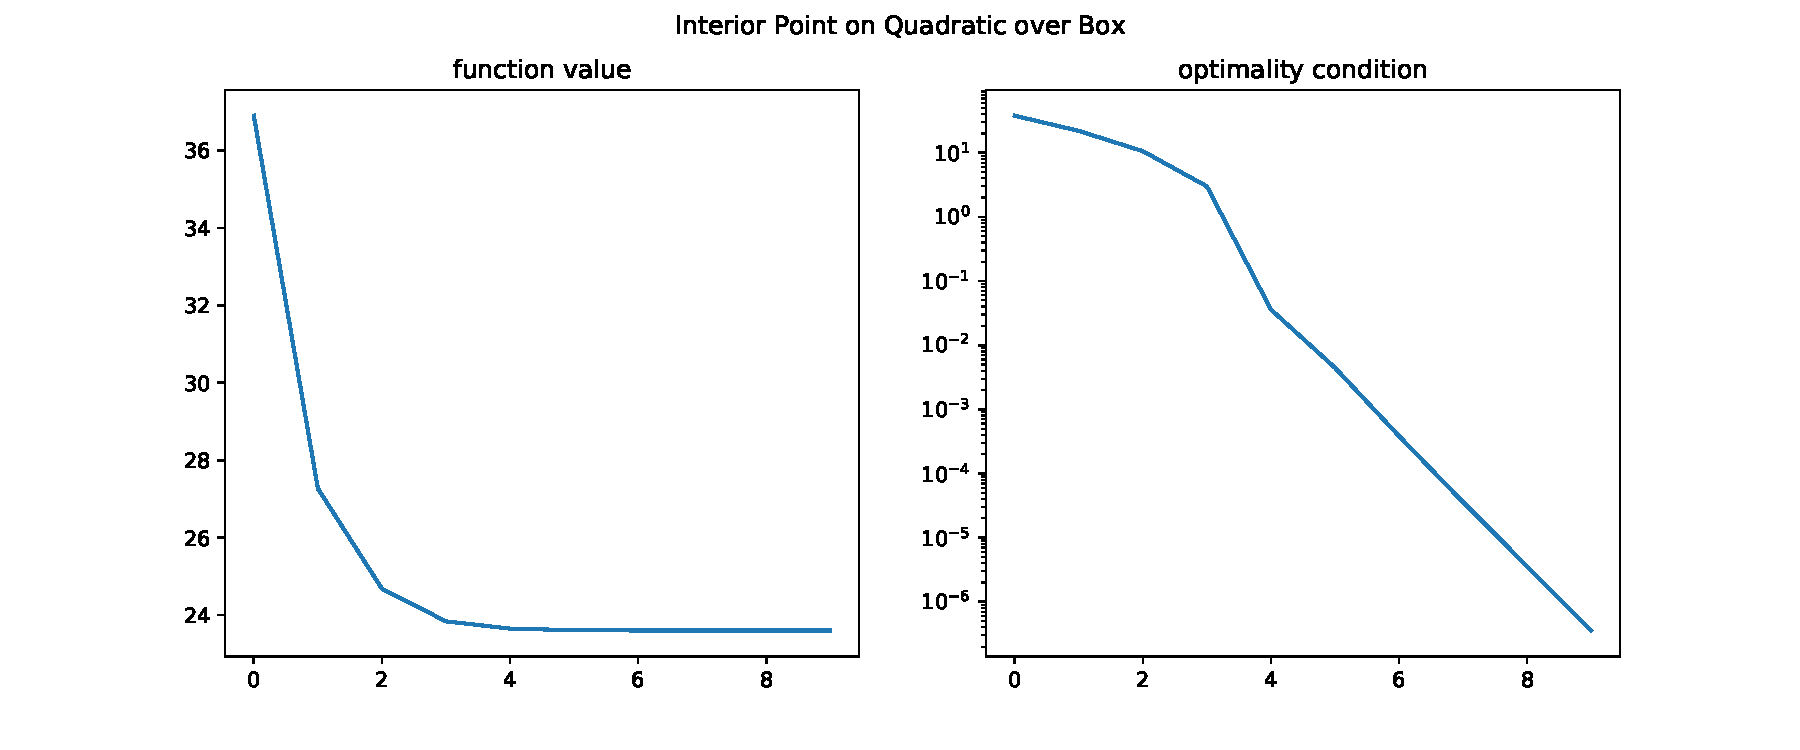
\includegraphics[width=\textwidth]{interior_point.pdf}
    \caption{Convergence of primal-dual interior point method.}
    \label{fig:interior_point}
  \end{figure}
\end{proof}



\item[(5)] Implement a Chambolle-Pock method to solve  
\[
\min_{x} \|Ax-b\|_1 + \|x\|_1. 
\]

\begin{proof}
  See \texttt{solvers.py} for the code and \texttt{515Hw4\_Coding.ipynb} for the
  demo. See Figure \ref{fig:signal_recovery} for a plot of the recovered signal.

  \begin{figure}
    \centering
    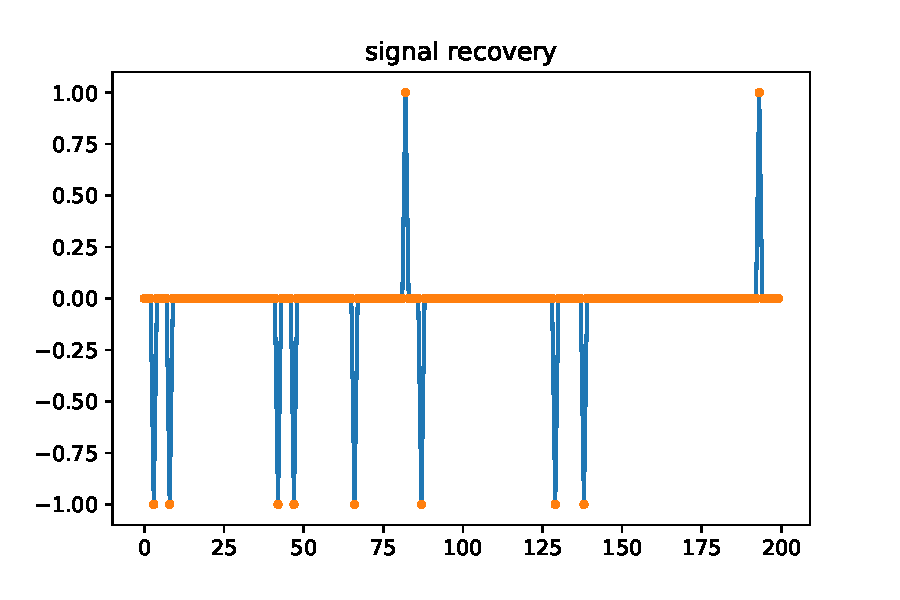
\includegraphics[width=\textwidth]{signal_recovery.pdf}
    \caption{Demonstration of the Chambolle-Pock recovering a signal.}
    \label{fig:signal_recovery}
  \end{figure}
\end{proof}



\end{enumerate}


\end{document}  
